\section{SIEM-Systeme}

\label{sec_state_siem}

Zur Zeit gibt es eine vielfältige Auswahl an SIEM-Systemen auf dem Markt, die die grundsätzlichen Aufgaben eines SIEM-Systems erfüllen und über diese hinausgehen: Splunk\footnote{
  https://www.splunk.com
}, QRadar von IBM\footnote{
  https://www.ibm.com/us-en/marketplace/ibm-qradar-siem
} oder ArcSight von Micro Focus\footnote{
  https://software.microfocus.com/en-us/software/siem-security-information-event-management
} sind nur einige Beispiele aus diesem Bereich. 

Die Auswahl an Open-Source-Software in diesem Bereich ist jedoch sehr gering. Eine der wenigen Ausnahmen stellt OSSIM - ein SIEM-System der Firma AlienVault\footnote{
	AlienVault OSSIM: The World’s Most Widely Used Open Source SIEM\\https://www.alienvault.com/products/ossim
} - dar, das auf Basis weiterer quelloffener Lösungen aus dem Netzwerksicherheits-Bereich unter anderem die in Abschnitt \ref{sec_basics_siem} beschriebenen Funktionen bereitstellt. AlienVault bietet zusätzliche eine kommerzielle Variante seines Produkts namens USM an, das insbesondere in den Bereichen Event-Korrelation und Compliance-Reporting die Funktionalität von OSSIM übersteigt. Von der Entwicklungsarbeit die in USM fließt, profitiert jedoch auch OSSIM, beispielsweise durch die Aktualisierung von Plugins für die Einbindung von aktuellen Netzwerkgeräten.

\subsection{OSSIM-Überblick}

\label{subsec_state_siem_overview}

Im Folgenden soll eine Übersicht über die für diese Arbeit relevanten Komponenten von OSSIM und deren Zusammenspiel gegeben werden. Diese ist auch in Abbildung \ref{fig:ossim_log_flow} dargestellt.

Den Kern des SIEM-Systems bildet der OSSIM-Server. Hier werden Events gespeichert sowie aggregiert und es findet die Korrelation von Events statt, die der Erkennung von Angriffen oder ungewöhnlichem Netzverhalten dient. Events und generierte Meldungen können über ein Web Interface betrachtet werden. Weiterhin können hier unter anderem Angaben zur Netzinfrastruktur bereitgestellt, Netzwerk- und Schwachstellenscanner bedient und sämtliche Informationen über den Netzwerkstatus eingesehen werden. 

Der OSSIM-Agent ist dafür zuständig, vorliegende Logdaten zu parsen und in ein OSSIM-spezifisches Event-Format zu übersetzen. Auf diesen Vorgang wird im nächsten Abschnitt genauer eingegangen. Die erzeugten Events werden anschließend an den Server weitergeleitet. Der Agent befindet sich sowohl direkt auf dem Server als auch auf jedem installierten Sensor. 

Eine OSSIM-Umgebung kann optional ein oder mehrere Sensoren nutzen, auf denen jeweils ein Agent seine Arbeit verrichtet. Dies wird im Folgenden verteilte Installation genannt. Der Vorteil dieser Lösung besteht darin, dass das aufwendige Parsen und Normalisieren von Logdaten verteilt staffinden und dadurch die Serverlast in großen Umgebungen reduziert werden kann. Kommt kein externer Sensor zum Einsatz, so spricht man von einer All-In-One-Installation.

\begin{figure}[]
    \centering
        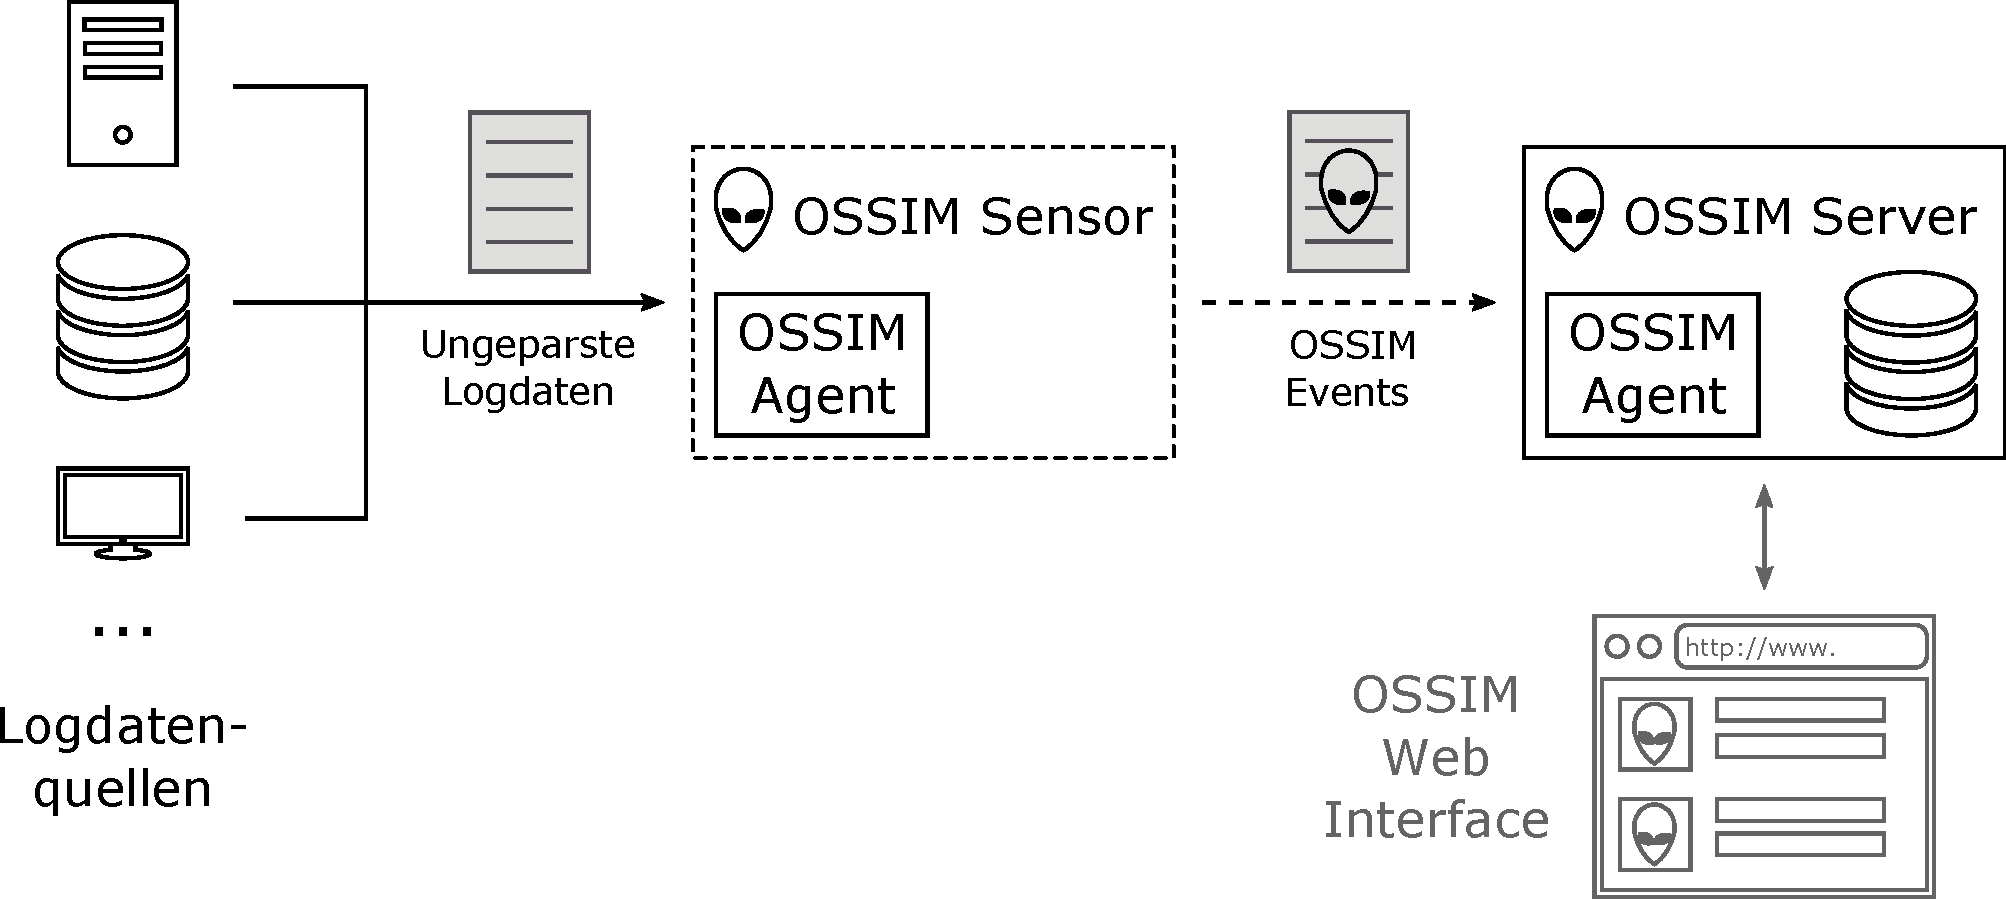
\includegraphics[width=0.9\textwidth]{dia/ossim_log_flow.pdf}
    \caption{High-Level-Übersicht über die OSSIM-Architektur und den Datenfluss.}
    \label{fig:ossim_log_flow}
\end{figure}


\subsection{Parsen von Logdaten in OSSIM}

\label{subsec_state_siem_parsing}

% Quellenarten
% Plugins
% OSSIM-Events
Besonders von Bedeutung für diese Arbeit ist die Verarbeitung von Logdaten. OSSIM ermöglicht es, Logdaten aus unterschiedlichen Quellen entgegenzunehmen bzw. aktiv selber abzurufen und in ein gemeinsames Event-Format zu übersetzen. Hierzu stehen verschiedene Möglichkeiten zur Verfügung:

\begin{itemize}
  \item Entgegennehmen von Daten über das Syslog-Protokoll
  \item Beschaffen von Daten über das SNMP-Protokoll
  \item Entgegennehmen von Daten über proprietäre Protokoll wie SDEE oder WMI
  \item Beschaffen von Daten durch Datenbankabfragen 
\end{itemize}

Unabhängig von der Datenquelle funktioniert die Verarbeitung der Logdaten nach dem immer gleichen Schema. OSSIM bietet die Möglichkeit mitgelieferte oder selber entwickelte Plugins für verschiedene Datenquellen zu aktivieren. Für eintreffende Logdaten überprüft der Agent anhand von regulären Audrücken, ob ein Plugin für das entsprechende Datum zuständig ist. Ist so ein Plugin gefunden, so wird ein neues OSSIM-Event angelegt und anhand der Angaben im Plugin die entsprechenden vorgegebenen Felder des Events gesetzt. Hierbei kann es sich beispielsweise um den Zeitpunkt des Events, IP-Adresse und Port der Datenquelle, einen zu dem Event gehörigen Netzwerkbenutzer oder ereignisabhängige selbstgesetzte Felder handeln. Anschließend folgt die Weiterleitung des Events an den Server.
